\documentclass[../../rapport/main]{article}
\usepackage[utf8]{inputenc}
\usepackage{blindtext}
\usepackage{amsmath,amsthm}
 \usepackage{amssymb}
%\usepackage{dsfont}                         % Enables double stroke fonts
\usepackage{color}
\usepackage[draft,inline]{fixme}
\usepackage[english]{babel}
\usepackage{graphicx}
\usepackage{float}
\usepackage{epstopdf}

\title{Determine ohmic resistance of motors}
\maketitle
\begin{document}
\section{Abstract}
The ohmic resistance of the two motors controlling the pan-tilt system gets determined.
\section{Introduction}
The ohmic ressitance of the motors are the goal to be determined in this jounal. Every constant concerning the motor of the topframe is denoted $A_t$ while constants for the buttom frame is denoted $A_b$.
\section{Materials and Methods}
To determine the ohmic resistance of the motors a known voltage will be applied, causing a current to flow through the motor. Using Ohm's law we thus can determine the wanted resistance.\\
The circuit used to determine the resistance fo the motor can be seen on figure (\ref{fig:resistance_circuit}). When executing the experiment a $VCC$ of $12V$ is chosen with a ohmic resistor with resistance $R_1 = 22\Omega$. Measuring the current flowing through the resistor in series with the motor on the top frame, its seen that $I_t \approx 0.449 A$.

\begin{wrapfigure}
  \label{fig:resistance_circuit}
  \begin{center}
    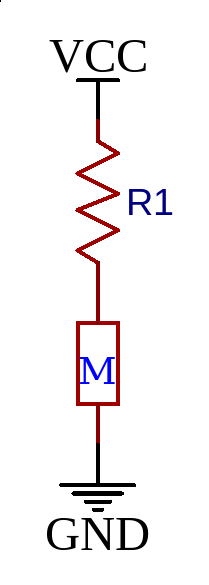
\includegraphics[width=0.1\textwidth]{screenshot-2019:05:08:12:43:17.png}
  \end{center}
\end{wrapfigure}
Doing the same but with the buttom frame, the current measured is $I_b \approx 0.448 A$. Thus the resistance of the two motors can be caluclated as:
$$VCC = (R_1 + R_{motor,t})\cdot I_t \Rightarrow R_{motor,t} = \frac{12V}{0.448 A}-22\Omega \approx 4.79 \Omega $$
$$VCC = (R_1 + R_{motor,b})\cdot I_b \Rightarrow R_{motor,b} = \frac{12V}{0.449 A}-22\Omega \approx 4.70 \Omega $$

\newpage

\section{Results}

The result of this experiment is as follows.
$$R_{motor,b} \approx 4.70 \Omega$$
$$R_{motor,t} \approx 4.79 \Omega$$

\section{Conclusion}

The resistance of the motor controlling the top frame is $R_{motor,t}\approx 4.79 \Omega$ and the resistance of the motor controlling the buttom frame is $R_{motor,b}\approx 4.70 \Omega$.










\end{document}
